% Appendix A

\chapter{Appendix A Planning Detailing} % Main appendix title

\label{AppendixA} % For referencing this appendix elsewhere, use \ref{AppendixA}

\section{Gantt Chart}

Figure \ref{fig:gantt_complete} presents a detailed Gantt chart that outlines all project sub-tasks and their respective timelines, showcasing the relationships and dependencies between tasks. While parallelism could potentially provide more time for individual tasks, achieving it in this project is challenging, as noted in the main document. However, a Start-to-Start relationship is established between the task of studying a language and the implementation or environment design. This decision reflects the importance of dedicating time to the study phase while allowing for parallel progress to optimize the schedule.

For clarity, the variance column has been omitted from the chart, as its details are thoroughly addressed in the main document. Similarly, the baseline, set at the project’s inception, has been excluded to avoid unnecessary visual complexity in the diagram.

\begin{figure}
    \centering
    \frame{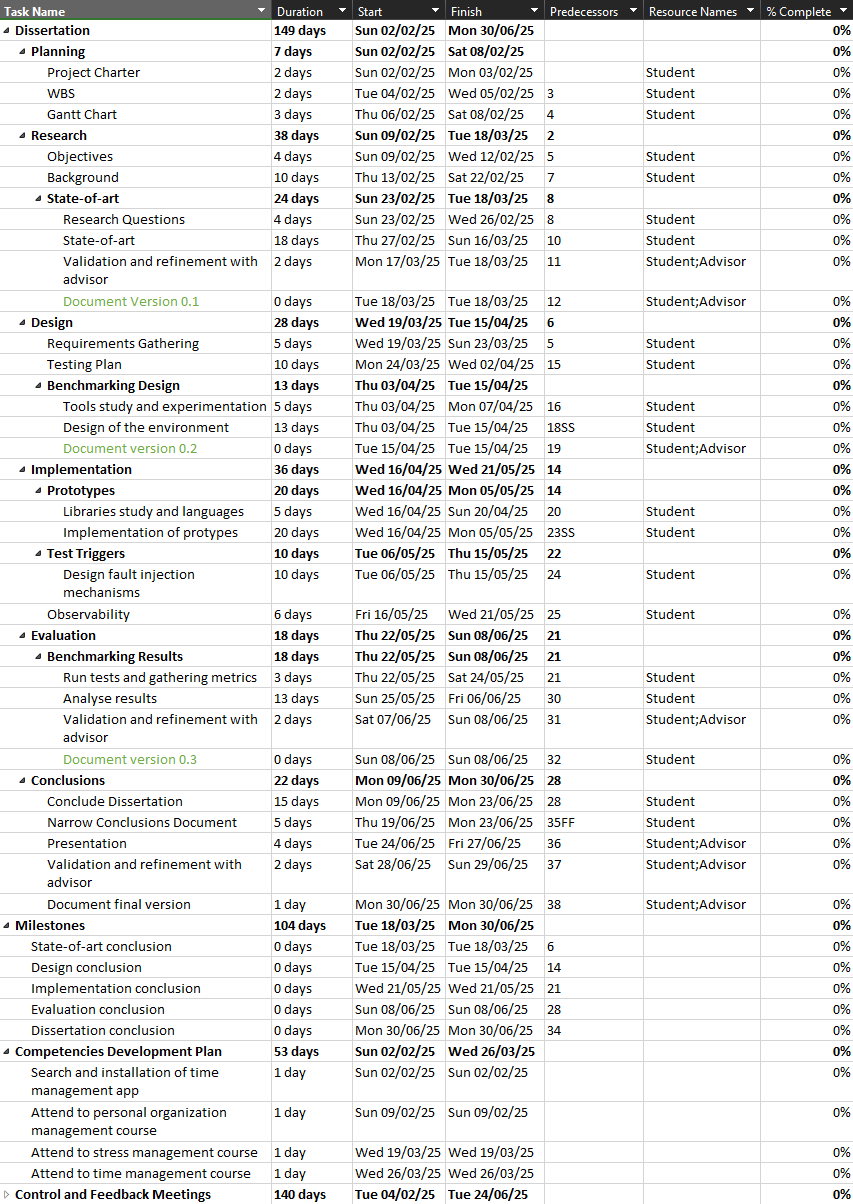
\includegraphics[width=\linewidth]{appendices/assets/gantt_complete.png}}
    \caption{Complete demonstration of the Gantt}
    \label{fig:gantt_complete}
\end{figure}

\section{Work Breakdown Structure Dictionary}

On the Table \ref{tab:wbs-dictionary} it is represented in a detailed way the description of the \gls{WBS}'s deliverables, such as the work loads. For each item there is a concise descriptions and a acceptance criteria.


\begin{longtable}{|p{3cm}|p{2.5cm}|p{8cm}|}
    \hline
    \textbf{Item Name}             & \textbf{Type of Item} & \textbf{Additional Description / Acceptance Criteria}                                                                                                                                                                                                                                                                                                     \\ \hline
    \endfirsthead
    \hline
    \textbf{Item Name}             & \textbf{Type of Item} & \textbf{Additional Description / Acceptance Criteria}                                                                                                                                                                                                                                                                                                     \\ \hline
    \endhead
    (1.1) Planning                 & Phase                 & This phase includes all initial project setup tasks.                                                                                                                                                                                                                                                                                                      \\ \hline
    (1.1.1) Project Charter        & Deliverable           & The project charter must be created following the project's scope and management guidelines. \newline \textbf{Acceptance Criteria:} The project charter must be approved by the advisor.                                                                                                                                                                  \\ \hline
    (1.1.2) \gls{WBS}              & Deliverable           & The \gls{WBS} should break down the project into manageable components. \newline \textbf{Acceptance Criteria:} The WBS should be validated by the advisor and include all project elements.                                                                                                                                                               \\ \hline
    (1.1.3) Gantt Chart            & Deliverable           & A detailed timeline outlining tasks, dependencies, competence development plan, milestones, and the dissertation deadline. \newline \textbf{Acceptance Criteria:} The Gantt chart must accurately reflect project phases and be reviewed by the advisor.                                                                                                  \\ \hline
    \hline 

    (1.2) Research                 & Phase                 & This phase focuses on gathering the required knowledge and literature to support the project.                                                                                                                                                                                                                                                             \\ \hline
    (1.2.1) Objectives             & Deliverable           & Clear objectives for the project, that must detail what are the excepted outcomes. \newline \textbf{Acceptance Criteria:} Objectives should align with the research goals and be validated by the advisor.                                                                                                                                                \\ \hline
    (1.2.2) Background             & Deliverable           & Research and summarize the background of fault tolerance in distributed systems and the distributed and concurrent programming languages.  \newline \textbf{Acceptance Criteria:} The background section should include sufficient theoretical content approved by the advisor, and must include a clear justification for the languages chosen.          \\ \hline
    (1.2.3) State-of-art           & Deliverable           & Review the current literature on fault tolerance in Elixir, Go, and Scala with Akka. Also, what are the latest techniques for benchmarking distributed and concurrent programming, and if there are already studies on this topic. \newline \textbf{Acceptance Criteria:} State-of-the-art review must highlight gaps and relevance to the project scope. \\ \hline
    \hline 

    (1.3) Design                   & Phase                 & This phase involves requirements gathering, testing plan, and benchmarking design.                                                                                                                                                                                                                                                                        \\ \hline
    (1.3.1) Requirements Gathering & Deliverable           & Collect requirements for the benchmarking and evaluation of fault tolerance aspects. \newline \textbf{Acceptance Criteria:} Requirements must be detailed, reviewed, and approved by the advisor.                                                                                                                                                         \\ \hline
    (1.3.2) Testing Plan           & Deliverable           & A plan for testing different fault tolerance strategies and mechanisms in Elixir, Go, and Scala with Akka. \newline \textbf{Acceptance Criteria:} Testing plan must include scenarios and validation methods, reviewed by the advisor.                                                                                                                    \\ \hline
    (1.3.3) Benchmarking Design    & Deliverable           & Define the design for benchmarking environments. \newline \textbf{Acceptance Criteria:} Benchmarking environments design must be validated by the advisor, and must adhere to the test plan created.                                                                                                                                                      \\ \hline
    \hline

    (1.4) Implementation           & Phase                 & This phase involves the development of benchmarking prototypes.                                                                                                                                                                                                                                                                                           \\ \hline
    (1.4.1) Prototypes             & Deliverable           & Develop prototypes in Elixir, Go, and Scala with Akka for fault tolerance testing. \newline \textbf{Acceptance Criteria:} Prototypes must meet the test plan previously created and must be supported on the benchmarking design planned.                                                                                                                 \\ \hline
    (1.4.2) Test Triggers          & Deliverable           & Create fault injection mechanisms for testing fault tolerance. \newline \textbf{Acceptance Criteria:} Fault injection methods must simulate real-world scenarios and be validated by tests.                                                                                                                                                               \\ \hline
    (1.4.3) Observability          & Deliverable           & Implement observability tools for monitoring system behavior during tests. \newline \textbf{Acceptance Criteria:} Observability setup must capture the metrics defined on the test validations methods.                                                                                                                                                   \\ \hline
    \hline 

    (1.5) Evaluation               & Phase                 & Evaluate the results of the benchmarking tests.                                                                                                                                                                                                                                                                                                           \\ \hline
    (1.5.1) Benchmarking Result    & Deliverable           & Analyze and document the outcomes of benchmarking fault tolerance aspects. \newline \textbf{Acceptance Criteria:} Results must be clear, reproducible, and reviewed by the advisor.                                                                                                                                                                       \\ \hline
    \hline 

    (1.6) Conclusions              & Phase                 & Finalize and present the results of the dissertation.                                                                                                                                                                                                                                                                                                     \\ \hline
    (1.6.1) Dissertation           & Deliverable           & Compile the dissertation document with findings and analyses. \newline \textbf{Acceptance Criteria:} Dissertation must meet academic formatting and content guidelines.                                                                                                                                                                                   \\ \hline
    (1.6.2) Conclusions            & Deliverable           & Write concise conclusions summarizing key findings from the research, with the goal of creating a guide for future developers consult. \newline \textbf{Acceptance Criteria:} Conclusions must be concise and detail what are the cons and pros of using each language for each specific case, so that develops can easily decide.                        \\ \hline
    (1.6.3) Presentation           & Deliverable           & Prepare and deliver the final presentation to the evaluation committee. \newline \textbf{Acceptance Criteria:} Presentation must be clear and precise.                                                                                                                                                                                                    \\ \hline
    \caption{\gls{WBS} dictionary}
    \label{tab:wbs-dictionary}
\end{longtable}